\documentclass[12pt]{article}
\usepackage{sbc-template} 
\usepackage{graphicx,url}
\usepackage{url}
\usepackage[brazil]{babel} 
\usepackage[utf8]{inputenc} 
\usepackage[T1]{fontenc}
\usepackage[normalem]{ulem}
\usepackage[hidelinks]{hyperref}

\usepackage[square,authoryear]{natbib}
\usepackage{amssymb} 
\usepackage{mathalfa} 
\usepackage{algorithm} 
\usepackage{algpseudocode} 
\usepackage[table]{xcolor}
\usepackage{array}
\usepackage{titlesec}
\usepackage{mdframed}
\usepackage{listings}

\usepackage{amsmath} 
\usepackage{booktabs}

\urlstyle{same}

\newcolumntype{L}[1]{>{\raggedright\let\newline\\\arraybackslash\hspace{0pt}}m{#1}}
\newcolumntype{C}[1]{>{\centering\let\newline\\\arraybackslash\hspace{0pt}}m{#1}}
\newcolumntype{R}[1]{>{\raggedleft\let\newline\\\arraybackslash\hspace{0pt}}m{#1}}

\newcommand\Tstrut{\rule{0pt}{2.6ex}} 
\newcommand\Bstrut{\rule[-0.9ex]{0pt}{0pt}} 
\newcommand{\scell}[2][c]{\begin{tabular}[#1]{@{}c@{}}#2\end{tabular}}

\usepackage[nolist,nohyperlinks]{acronym}

\title{Real Time Detection of Pump-and-Dump Schemes in Cryptocurrency Markets}

\author{Matheus Moura\inst{1}}


\address{Centro Federal de Educação Tecnológica Celso Suckow da Fonseca - CEFET/RJ
	\email{matheus.moura@aluno.cefet-rj.br}
}



\begin{document} 
	
	\maketitle
	
	\begin{resumo} 
		Este roteiro traz as principais informações para a elaboração de trabalhos científicos. o trabalho deve ser escrito de modo a se mostrar interessante e importante. Para tanto, a forma de escrevê-lo, principalmente no resumo e  introdução, é fundamental. É o momento no qual o autor deve ``vender o trabalho''. 
		
		Em textos científicos, as frases devem ser curtas, para não gerar ambiguidade. Pode-se dizer que um parágrafo é constituído por pelo menos três frases. Adicionalmente, pode-se dizer que cada parágrafo tem uma única ideia central, \emph{i.e.}, uma sentença  que sumariza o parágrafo. 
		
		O texto de um trabalho todo precisa estar encadeado \citep{zobel_writing_2015}. O encadeamento dos parágrafos é feito a partir do encadeamento de suas ideias centrais. Desta forma, a ideia central de cada parágrafo leva a ideia central do próximo e assim por diante. 
		
		Em linhas gerais, qualquer parágrafo do trabalho que não apresente citação é considerado criação dos autores. A utilização de textos transcritos de alguma fonte sem a devida referência a esta fonte e seus autores pode configurar a hipótese de plágio. Assim, todas as obras citadas devem ter as referências aos seus autores e devem figurar na lista de referências do trabalho.
	\end{resumo}
	
	\section{Introdução}
	\label{sec_introducao}

	The adoption of cryptocurrencies has experienced significant growth over the past decade, leading to a substantial expansion of the market both within traditional financial sectors and in public perception.
	This trend is exemplified by notable milestones, such as the approval of the first Bitcoin futures Exchange-traded fund (ETF) by the U.S. Securities and Exchange Commission (SEC) in 2021 \citep{wursthorn2021} and the trading commencement of spot ETFs on American stock exchanges in early 2024 \citep{schmitt2024}.
	The surge in public interest can be attributed to the exponential growth observed in the cryptocurrency market during late 2017 and early 2018, which captured widespread attention from mainstream media, attention that recurs with each subsequent occurrence of high bullish market trends \citep{steinmetz2021}.
	Consequently, there is a pressing need for comprehensive studies to assess the risks associated with this fairly new asset class.

	The vast majority of cryptocurrencies operate without reliance on any central authority and offer a degree of anonymity.
	These features facilitate their utilization in illicit activities, including but not limited to money laundering, drug trafficking, and hacking \citep{Kethineni2019}.
	Among the various fraudulent practices associated with cryptocurrencies, one prominent scheme is the pump-and-dump (P\&D) tactic, characterized by the artificial inflation of an asset's price followed by the sale of the acquired assets at a higher price \citep{li2021}.

	Organizers of pump-and-dumps leverage on social media platforms that offer some level of anonimity, such as Telegram and Discord.
	Where they establish a public group or channel and recruit as many members as possible for what are colloquially termed "pump groups".
	Within these groups only scheme organizers are allowed publishing messages and once a critical mass of members is attained, typically exceeding 1,000, operations commence \citep{xu2019}.

	The typical modus operandi of "pump groups" starts with the dissemination of precise details, including the exact date, time, and exchange where the pump-and-dump operation will occur, allowing members adequate time to prepare their funds.
	At the pre-arranged time, the group administrators announce the targeted cryptocurrency and encourage members to acquire and retain it to artificially inflate its price.
	Throughout the pumping phase, participants promote the targeted coin on social media platforms to attract external attention.
	However, in a few minutes the price peak is reached and the participants begin panic-selling at the first sign of decline, leading to a rapid return of the coin's price to its pre-pump level \citep{xu2019}.
	
	Assim como o resumo de um trabalho pode ser entendido como uma vitrine, a introdução pode ser comparada a sala de estar do trabalho. A partir dela que o leitor deve decidir se o seu projeto final é interessante e se ele lerá o resto do seu trabalho. Desta forma, a escrita da introdução é fundamental, devendo se apresentar de modo bem encadeado. 
	
	Estruturalmente a introdução é constituída pela motivação, definição do problema, objetivos, principais resultados alcançados e estrutura do trabalho, mas estes elementos não aparecem de modo explícito no texto, \emph{i.e.}, a introdução não deve ter subseções. O leitor observa a presença destes elementos durante a leitura a partir do encadeamento do texto. Não existe uma regra para o número de parágrafos para cada um destes elementos. A motivação, por exemplo, pode ter vários parágrafos. A regra básica é que cada parágrafo tenha apenas uma ideia central e estas ideias levem a formulação da motivação. 
	
	A motivação deve apresentar a importância e justificar a escolha do tema do seu trabalho. Pode ser entendida como o motivo da escolha do tema do trabalho. A explicação deve conter a importância do conteúdo do trabalho, ou a oportunidade de criação de uma utilidade do trabalho, ou a viabilidade de desenvolvimento do trabalho de tema do trabalho, deixando claro que existem lacunas que podem ser mais bem exploradas. 
	
	A definição do problema pode ser entendida como a definição precisa do problema a ser tratado pelo trabalho, visando atender algum problema levantado na motivação. A definição não precisa se aprofundar em detalhes, mas deve ser feita de forma clara e objetiva, visando a expor a natureza do trabalho realizado. A definição do problema demonstra a intenção do trabalho, apresentando o assunto do trabalho de forma geral, mas motivadora para o leitor. Ela deve ser feita logo no início do trabalho caracterizando o mesmo. Porém, seu conteúdo deve ser revisto ao término do trabalho, para deixá-lo compatível com o trabalho realizado.
	
	Os objetivos são as metas a serem atingidas pelo trabalho. Comumente faz parte dos objetivos estabelecer uma solução para a definição do problema. Ela pode caracterizar em uma visão de alto nível, a abordagem adotada para abordar o problema definido. Podemos classificar os objetivos como: objetivo geral e objetivos específicos. No objetivo geral temos a meta principal do trabalho, respondendo o porquê do tema do trabalho. Nos objetos específicos temos a definição das metas individuais e sequenciais para atingir o objetivo geral. Neste momento, as contribuições devem ser elencadas e explicitadas.
	
	A estrutura do trabalho é comumente apresentada no último parágrafo da introdução. Cabe salientar que um trabalho não é um romance, isto é, não devem aparecer elementos surpresas ao longo do texto. O texto é elaborado e apresentado de modo bem organizado e planejado. 
	
	\section{Fundamentação Teórica}
	\label{sec_fund_teorica}
	
	A fundamentação teórica apresenta os principais conceitos relacionados ao domínio do problema. Não é objetivo da fundamentação teórica apresentar um conhecimento novo. O objetivo é caracterizar o domínio do problema, apresentando os principais conceitos que viabilizem o desenvolvimento de uma solução. Pode ser entendida como a fundamentação teórica, \emph{i.e.}, conceitos teóricos computacionais e científicos utilizados no desenvolvimento do trabalho.
	
	Este capítulo pode ter várias subseções, uma para cada diferente tema abordado. Por exemplo, se o objetivo do projeto final for implementar um jogo computacional de competição em ferramentas de redes sociais, pode-se ter uma subseção tratando os jogos computacionais e seus aspectos e posteriormente outra subseção tratando de redes sociais. Esta organização deve ser bem definida, mas o princípio básico do bom encadeamento deve ser preservado.
	
	
	As Figuras, Tabelas e Equações devem ser numeradas e citadas no texto. A Tabela \ref{tab_exemplo} apresenta um exemplo de tabela. A Figura \ref{fig_exemplo} apresenta um exemplo de figura. A Equação \ref{eq_exemplo} apresenta um exemplo de equação. Cada figura, tabela e equação merece um parágrafo de explicação própria.
	
	\begin{table}[!ht]
		\centering
		\caption{Exemplo de tabela}
		\begin{tabular}{L{1.5cm} R{1.5cm}}
			\toprule
			\textbf{x}  & \textbf{y} \\
			\midrule
			-2  & 4 \\
			-1  & 1 \\
			0  & 0 \\
			1  & 1 \\
			2  & 4 \\
			\bottomrule
		\end{tabular}
		\label{tab_exemplo}
	\end{table}
	
\begin{figure}[!ht]
 \centering
 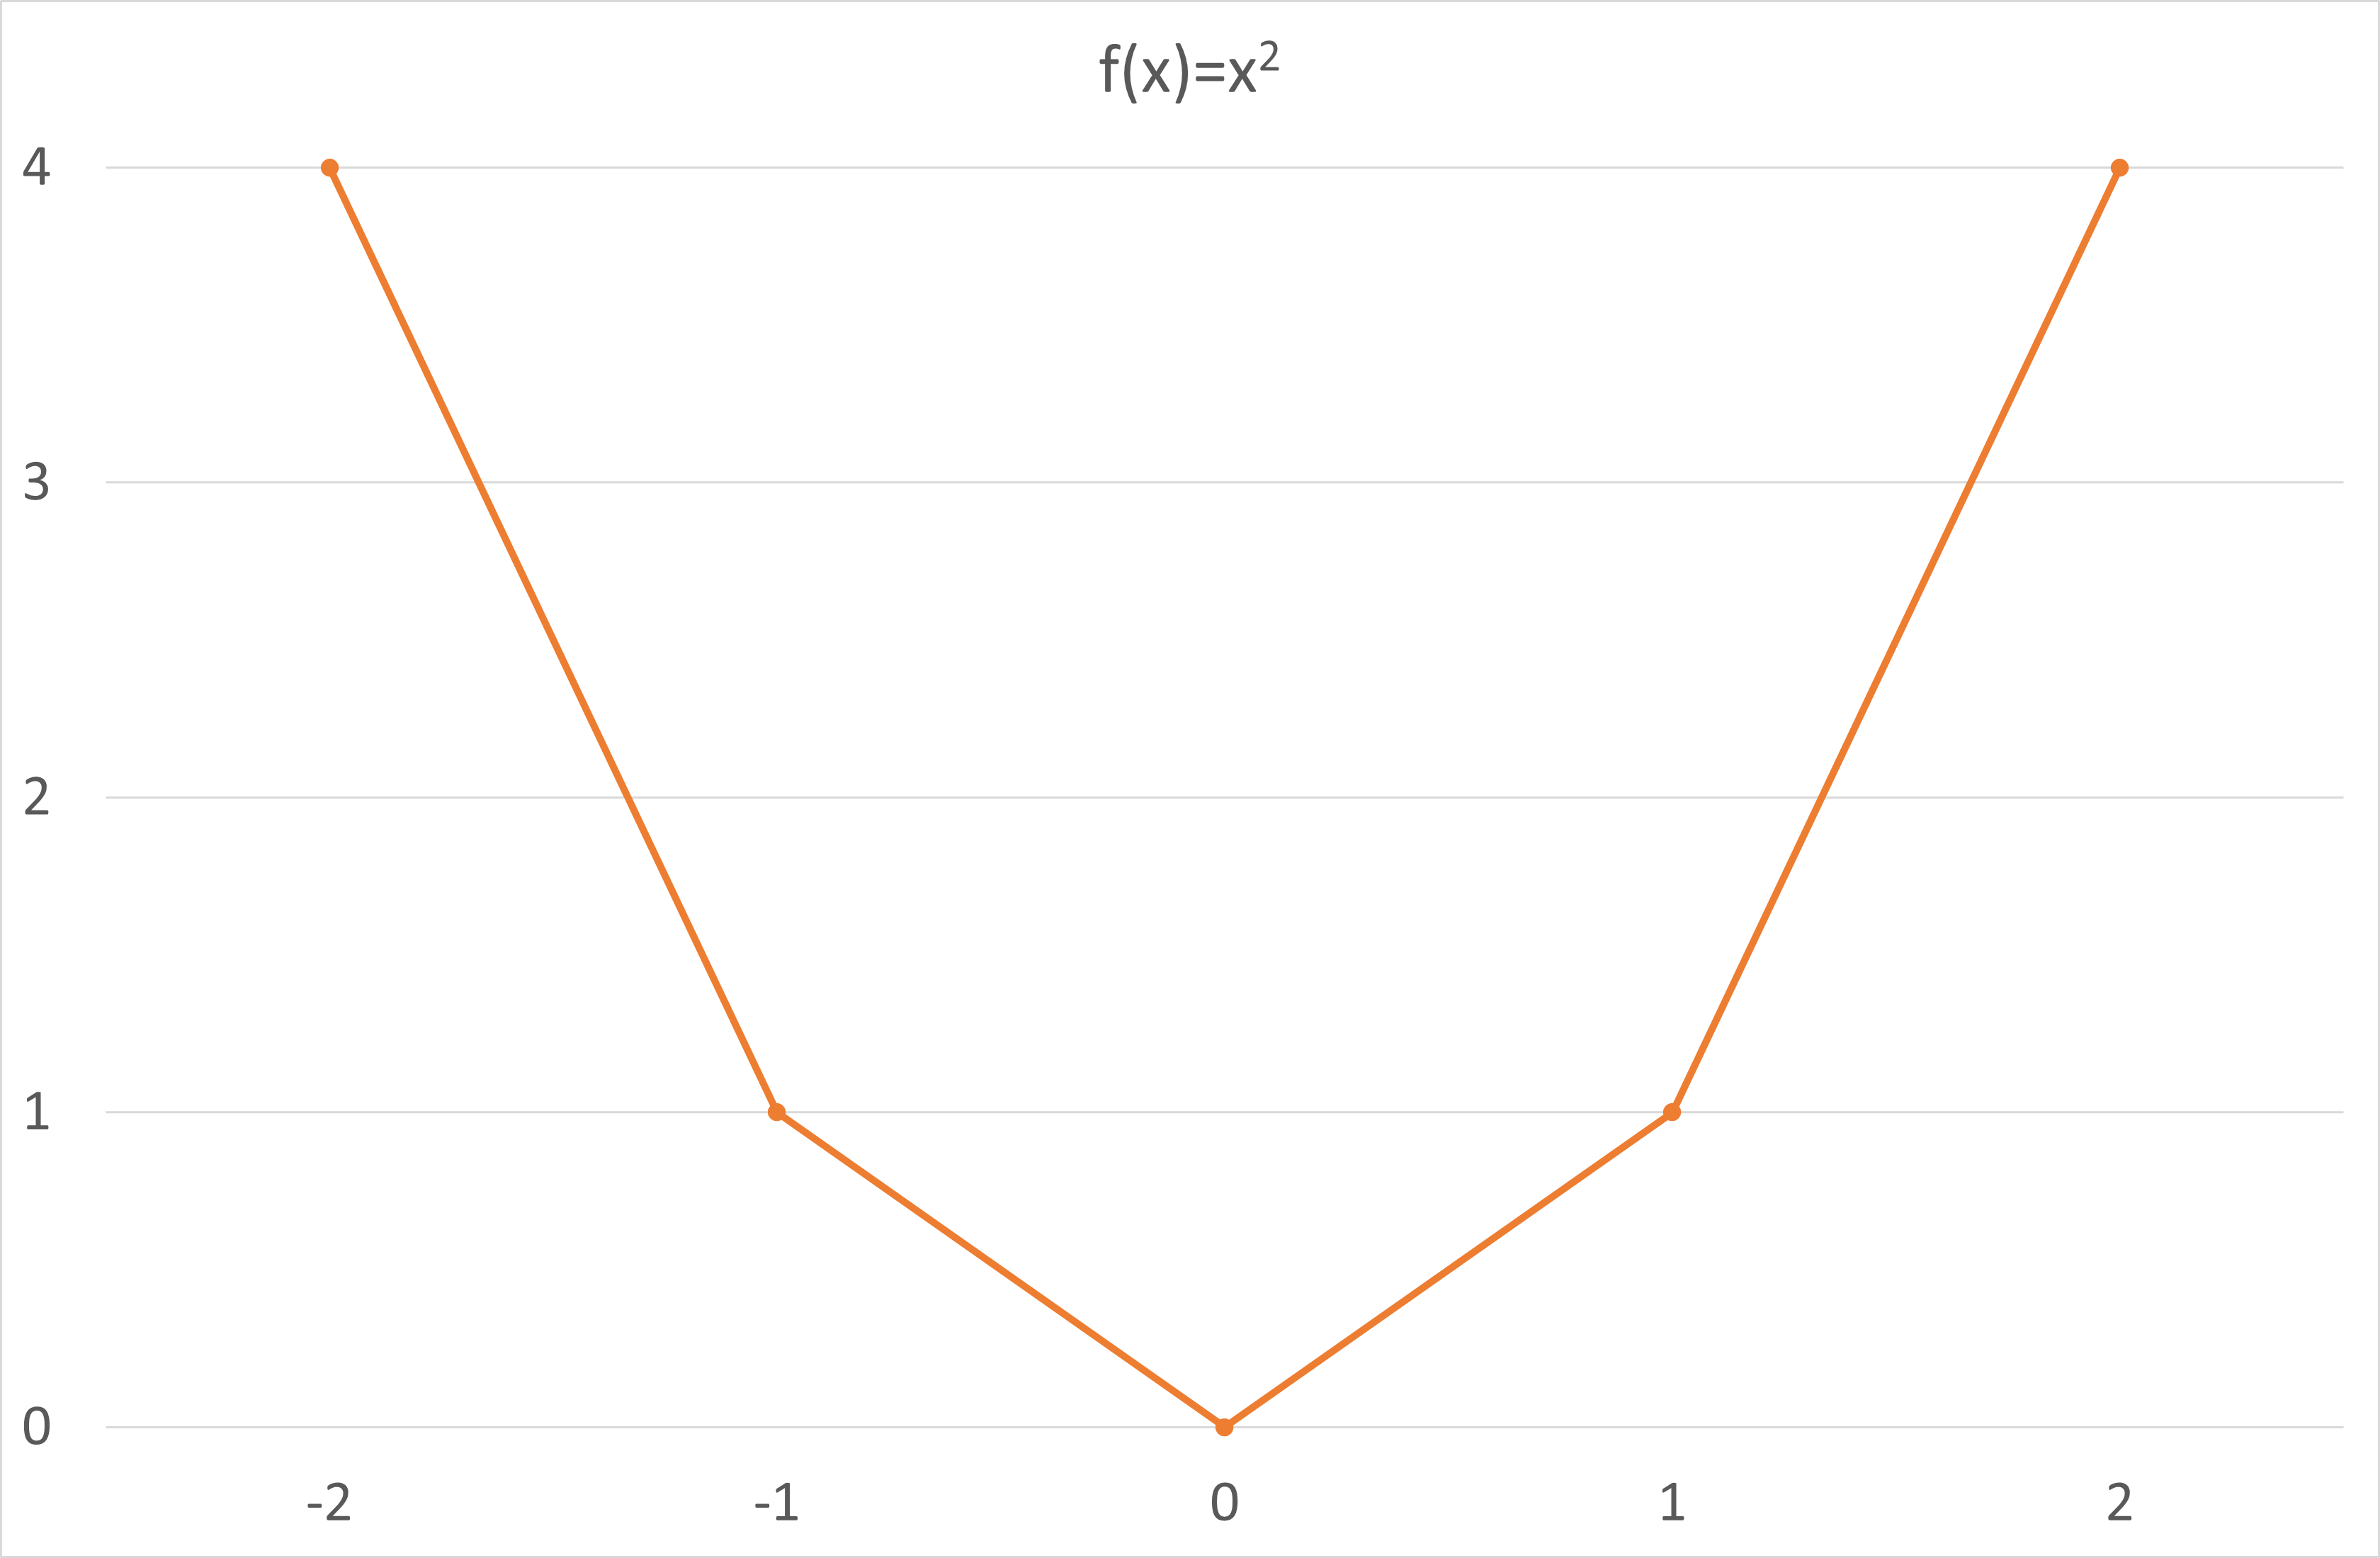
\includegraphics[width=0.6\textwidth]{figures/figura.png}
 \caption{Exemplo de figura}
 \label{fig_exemplo}
\end{figure}	

\begin{equation}
\label{eq_exemplo}
 f(x) = x^2, x \in [-2,2]
\end{equation}


	
	
	\section{Trabalhos relacionados}
	\label{sec_trab_relacionados}
	
	Ao final da fundamentação teórica devem ser apresentados os trabalhos relacionados referentes soluções semelhantes para o problema definido. Os trabalhos relacionados demonstram o estado da arte do tema do trabalho \citep{wazlawick_metodologia_2017}. Descrevemos, resumidamente, os trabalhos e pesquisas já efetuados na área do tema do trabalho, indicando os estudos realizados e os resultados obtidos por seus autores. Esta elaboração deve ser obtida a partir de um mapa sistemático\footnote{Eventualmente esta seção pode ficar depois da avaliação experimental}. 
	
	\section{Método}
	\label{sec_metodo}
	
	O desenvolvimento, juntamente com a avaliação experimental, é um dos núcleos do trabalho. O desenvolvimento compreende a modelagem e a elaboração da solução propriamente dita. Deve ser apresentado de forma ordenada e ampla, com o conteúdo relevante para a apresentação da solução a que o trabalho se propõe. Fica a cargo dos autores estabelecer a estrutura deste capítulo, bem como definir os elementos que devem ser utilizados para elaborar o desenvolvimento da solução. 
	
	A modelagem da solução para a elaboração dos artefatos computacionais define os principais elementos que fazem parte da solução proposta pelo trabalho. Em um sistema de informação, por exemplo, é natural a presença de um diagrama arquitetura, diagrama de caso de uso, um diagrama de classes. Na existência de um processo importante, pode-se recorrer a um diagrama de atividades. Da mesma forma, na existência um procedimento computacional complexo, pode-se fazer valer de especificação de um algoritmo em pseudocódigo, de diagrama de sequência, dentre outros, para explicá-lo. É importante deixar claro que o foco não é volume de elementos de diagramação e diferentes tipos de modelo, mas sim a qualidade da explicação da solução.
	
	A qualidade da explicação está intimamente ligada ao bom encadeamento deste capítulo. Isso significa dizer que se um diagrama for incorporado neste capítulo, cada elemento do diagrama precisa ser explicado. Por exemplo, se for utilizado um diagrama de classe, as principais classes e atributos devem ser apresentados, uma vez que cada uma das classes e cada atributo deve ser explicado no texto.
	
	A elaboração da solução propriamente dita apresenta um detalhamento dos elementos da solução. Pode envolver a especificação da arquitetura da solução, projeto lógico e físico da base de dados, projeto de interface gráfica, linguagem de programação adotada como os seus respectivos \emph{frameworks}. Novamente, o nível de detalhamento dos elementos da solução deve estar condizente com a explicação textual. Não é necessário apresentar todos os elementos da solução. O importante é deixar claro os elementos que valorizem a contribuição do trabalho.
	
	\section{Avaliação experimental}
	\label{sec_aval_exp}
	
	A avaliação experimental compreende uma avaliação quantitativa ou qualitativa do trabalho a partir de critérios estabelecidos para comparação. Como em qualquer experimento, a capacidade de reprodução é fundamental para sua validade. Sendo assim, é importante descrever o processo de experimentação adotados, apresentar os resultados propriamente dito, com uma síntese explicativa dos principais resultados. Finalmente, devem ser apresentadas as ameaças ao estudo, \emph{i.e.}, qualquer coisa que possa tirar ou limitar a validade do experimento conduzido. 
	
	\section{Conclusão}
	\label{sec_conclusao}
	
	A conclusão é a finalização do trabalho e indica as conclusões obtidas com o desenvolvimento do trabalho, sejam elas positivas ou negativas. Nas conclusões, analisa-se o que era desejado (definido na introdução com os objetivos), comparando com o alcançado pelo trabalho, descrevendo como os objetivos foram alcançados e o porquê de algum objetivo não ter sido alcançado. Destacam-se também as contribuições do trabalho, incluindo os benefícios e inovações trazidas pelo trabalho.
	
	Apresentam-se os pontos do trabalho que merecem um maior aprofundamento de estudos. Isso possibilita a criação de novos trabalhos com estudos nesses pontos apresentados, na forma de uma continuidade das pesquisas efetuadas pelo trabalho. Os trabalhos futuros indicam, ainda, uma maturidade de pesquisa do autor do trabalho e esses pontos podem ser trabalhados, posteriormente.
	
	\section*{Agradecimentos}
	Agradecimento as agências de fomento\footnote{Lembre-se de agradecer a CAPES se você tiver usado o Portal de Periódicos}.
	
    \bibliographystyle{apalike}
	\bibliography{references}
	
\end{document}
